\chapter{Regionally Containing Epidemics \RNum{2}: Modelling Ash dieback}

\section{Plant-based reproduction ratios, $R_0$}

\begin{itemize}
    \item see for a review on how R0 is calculated \cite{perspectives-on-r0}, we use method x in order to estimate and inform R0
    \item $R_0$ is a complex function which changes in time, to this end, the next generation operator is used to derive a value for $R_0$ \cite{doi:10.1098/rsif.2009.0386}. In order to inform the value of $R_0$ we do xy and z...
    \item Although it is hard to enforce a true $R_0$ value, the most important feature introduced from the definition is a threshold from which we can see if a local invasion is likely to take place.
    \item Since the number of susceptible hosts is fixed, without replacement, the number of susceptible hosts will continually decrease in time in the case of an epidemic. Given the strong spatial component in the model we expect that measuring $R_0$ as-per this definition will give an under-estimate for later times when few susceptible trees remain. Likewise, for earlier times when susceptible neighbours are plentiful $R_0$ will yield an upper estimate for the pathogen. In order to characterise the pathogen in this model, we take the upper bound defined between the $1^{st}-2^{nd}$ generations. This simplification represents a worst-case scenario and the mean value of $R_0$ would be lower for later times when there are less trees available to infect. But most importantly, the threshold of transmission $R_0>1$ is reliable captured \textit{during the initial stage of infection}.
    \item $R_0$ can be fully characterised by a growth rate \cite{R0-construct}. That is, the growth factor per generation.
    
\end{itemize}

\textcolor{red}{Fill with a mini lit review on $R_0$}

\textcolor{red}{Improvements to Chapter \ref{chapter:regional-containment1}}
\begin{enumerate}
    \item Lack of biological specificity. We choose Ash dieback% why not OAK?
    \item Informed dispersal kernel at the local-scale $\approx 1.6\mathrm{km}$
    \item Re-defined $R_0$
    \item $\beta$ between to limits
    \item Course-grained $R_0$ map to $5-10\mathrm{km^2}$
    \item Inclusion of power-law dispersal
    \item Are results different ?
    \item to our knowledge $R_0$ has not been estimated for Ash dieback but has been for wheat strip rust \cite{segarra2001epidemic}
\end{enumerate}

In this Chapter aspects of the sub-grid model are improved.//
\section{The biology of Ash dieback} % why not remain with Oak?
\begin{itemize}
    \item review: \cite{ash-dieback-costs}
    \item review: \cite{doi:10.1111/1365-2745.13383}
    \item review: \cite{ash-tree1}
\end{itemize}

\section{Model improvements...}
\begin{itemize}
    \item \textcolor{red}{At the small scale we have a uniform population. However for larger scales we have considerable spatial heterogeneity.}
    \item some regions can sustain an epidemic and some cannot, we assume that $R_0>1$ is the threshold separating these regimes.
    \item Looking at \cite{R0-perc-ref}, it makes me think our notion of $R_0$ is pretty simplistic. We only measure the local-level $R_0$. We do not consider $R_0$ from patch to patch. What scale we measure $R_0$ has a huge impact on what the result is. Could we rank land-patches not only on there local $R_0$ level, but also on the impact they have on there immediate neighbours ? This would, in theory be an improvement to the clustering algorithm.
    \item The algorithm to target not only the critically connecting patches, but also find fragmenting lines which minimise risk at the landscape-level ? Incorporating the local impact a particular patch may have on its neighbours.
    \item introduce the regime of pathogen spread we are interested in, we are not modelling continental long-range spread via upper atmosphere, nor are we interested in long-range human trade networks. We are interested in dispersal at the local level whereby passive means of wind, soil and or insects/animals. 
    
    
\end{itemize}
From a brief investigation of the newly-defined, %
and more realistic, $R_0$ value, we can produce a new $R_0$-map. %
However, time using the dispersal kernel of ash dieback is informed from data. Dispersal is found to be on the order of $\approx 1\mathrm{km^2}$. This stands in contrast to the value of $25\mathrm{m}$ that we choose in Chapter \ref{chapter:regional-containment1}.

\begin{figure}
    \centering
    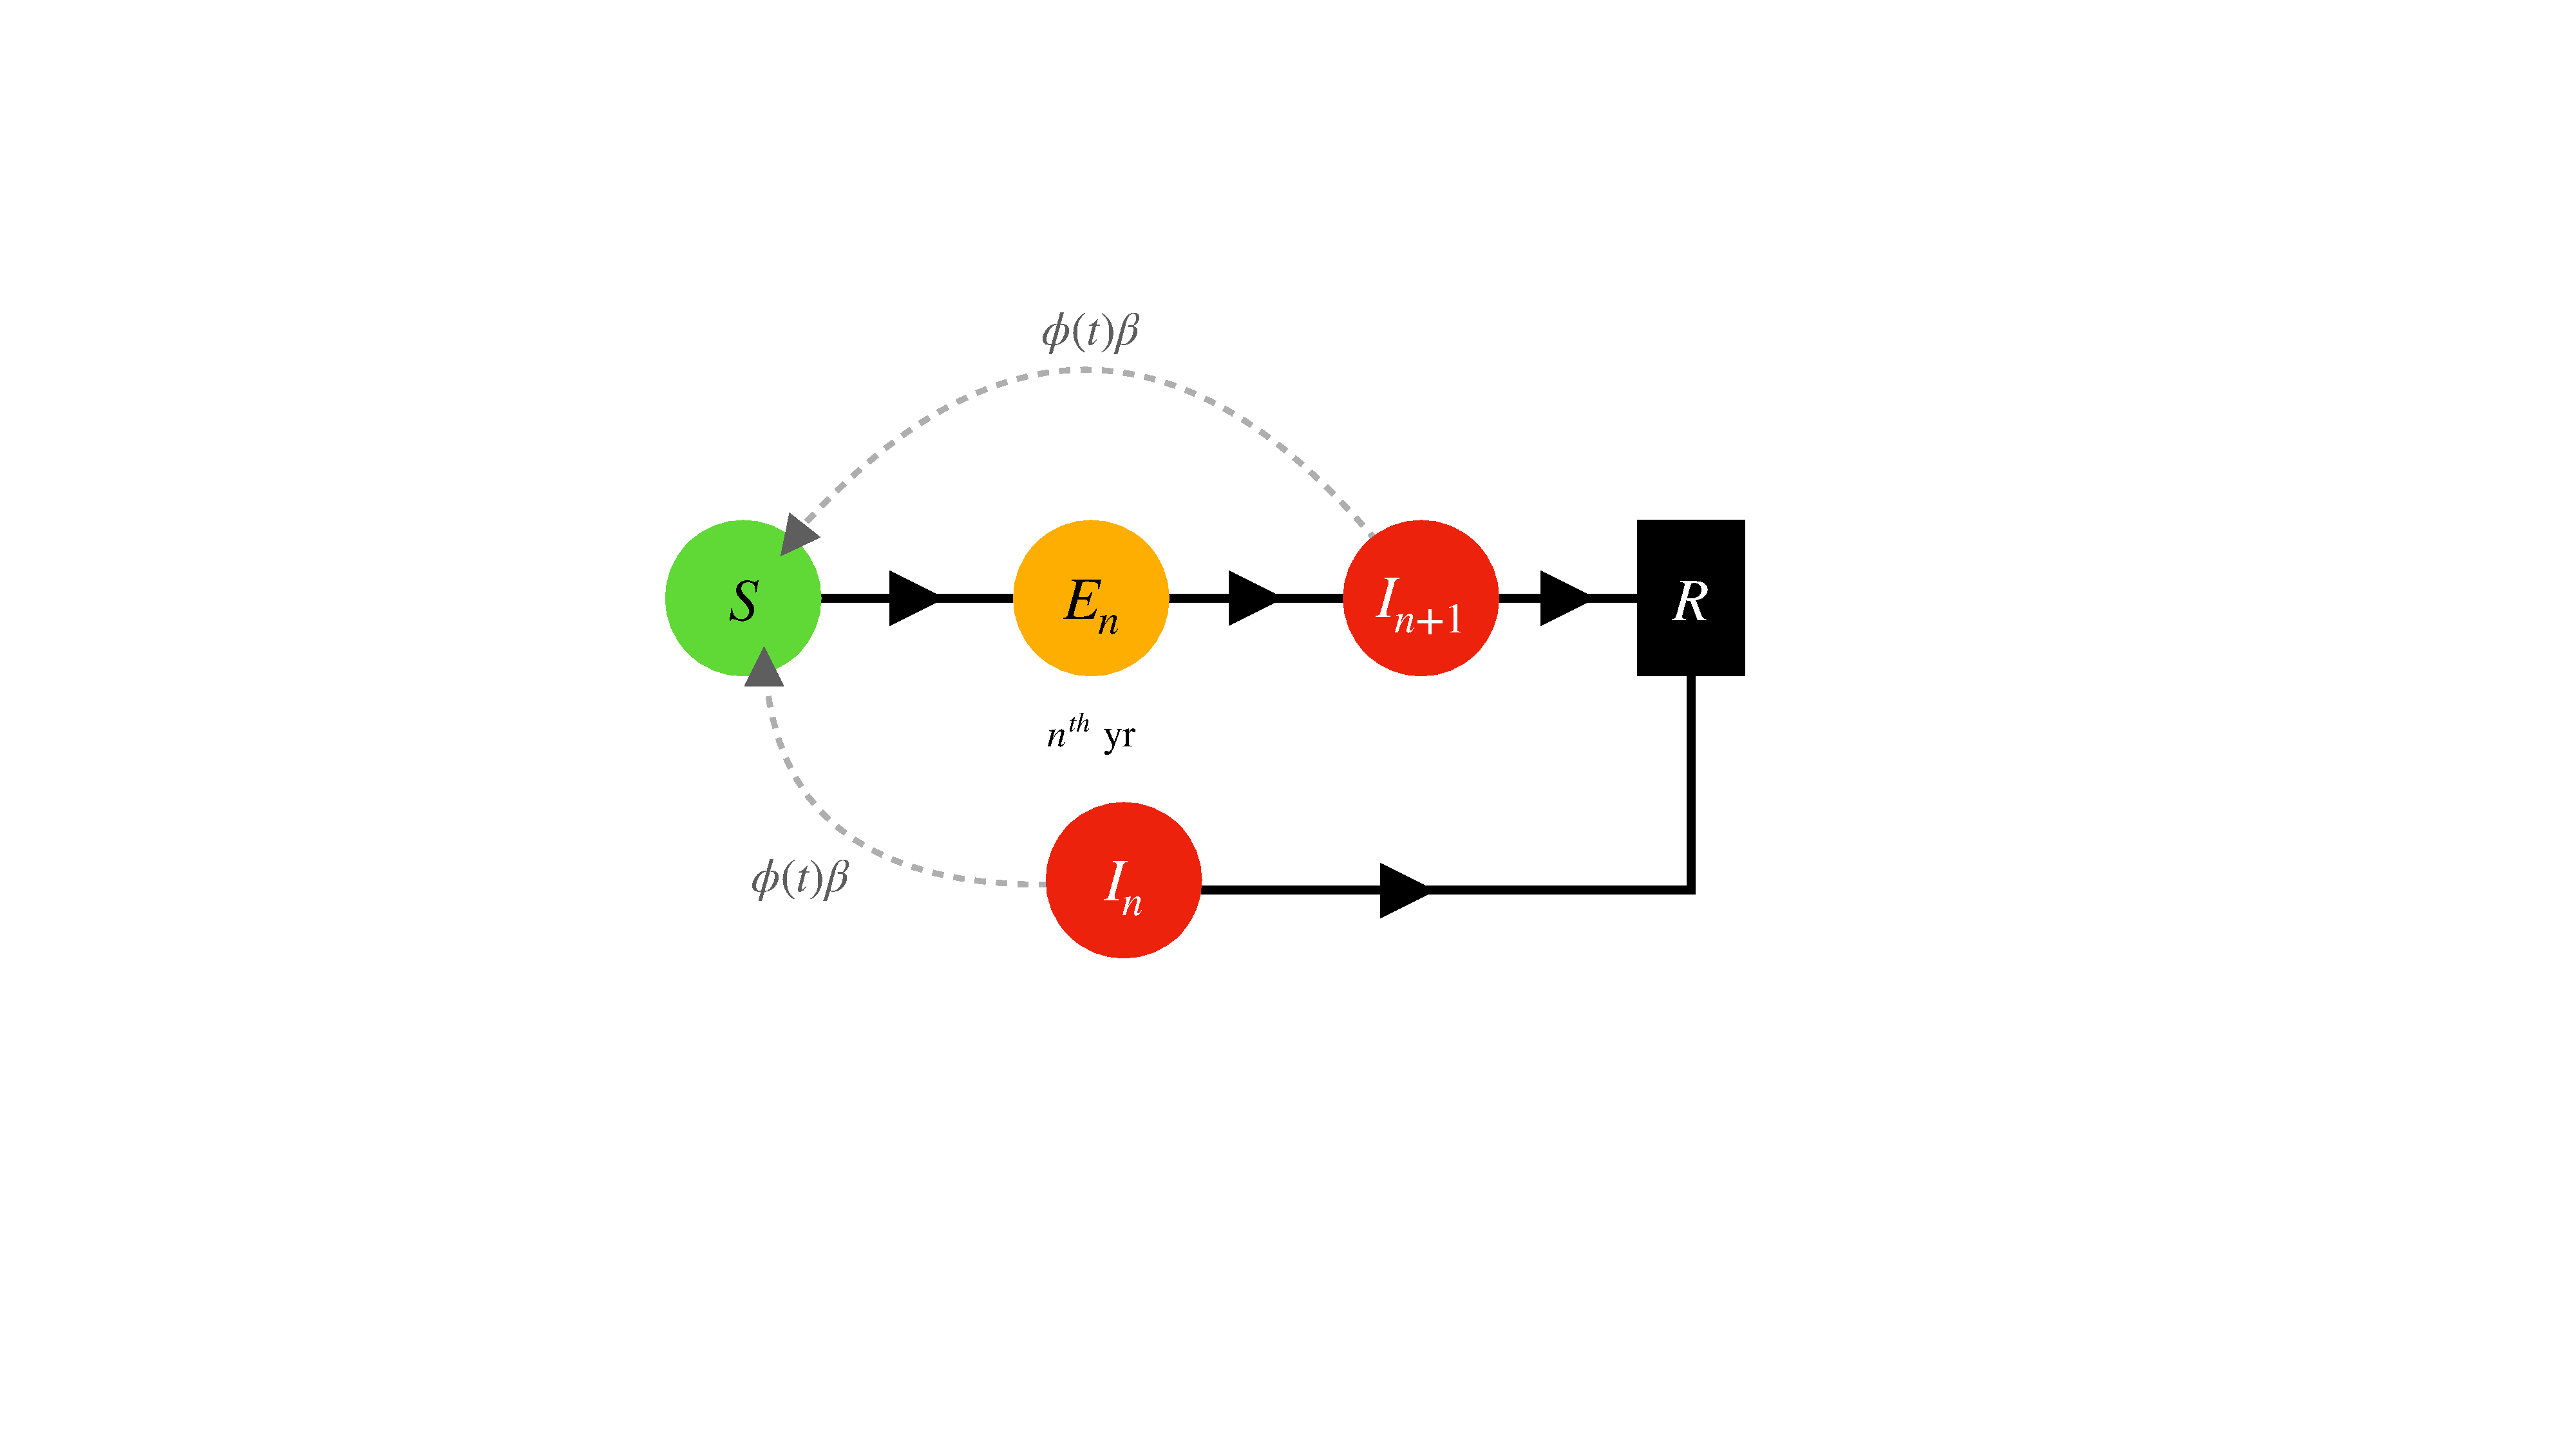
\includegraphics[scale=0.30]{chapter6/figures/fig1.pdf}
    \caption{Contact-traced $R_0$, the 'true' $R_0$. Tracking the history of all infected trees allows us to count how many infections are produced for each infectious tree over a simulation. At $t=0$, a handful of ($0^{th}$-generation) infections are positioned randomly throughout the domain. The quantity $R_0$ is defined as the mean number of secondary infections produced over all generations.}
    \label{fig:my_label}
\end{figure}

\begin{figure}
    \centering
    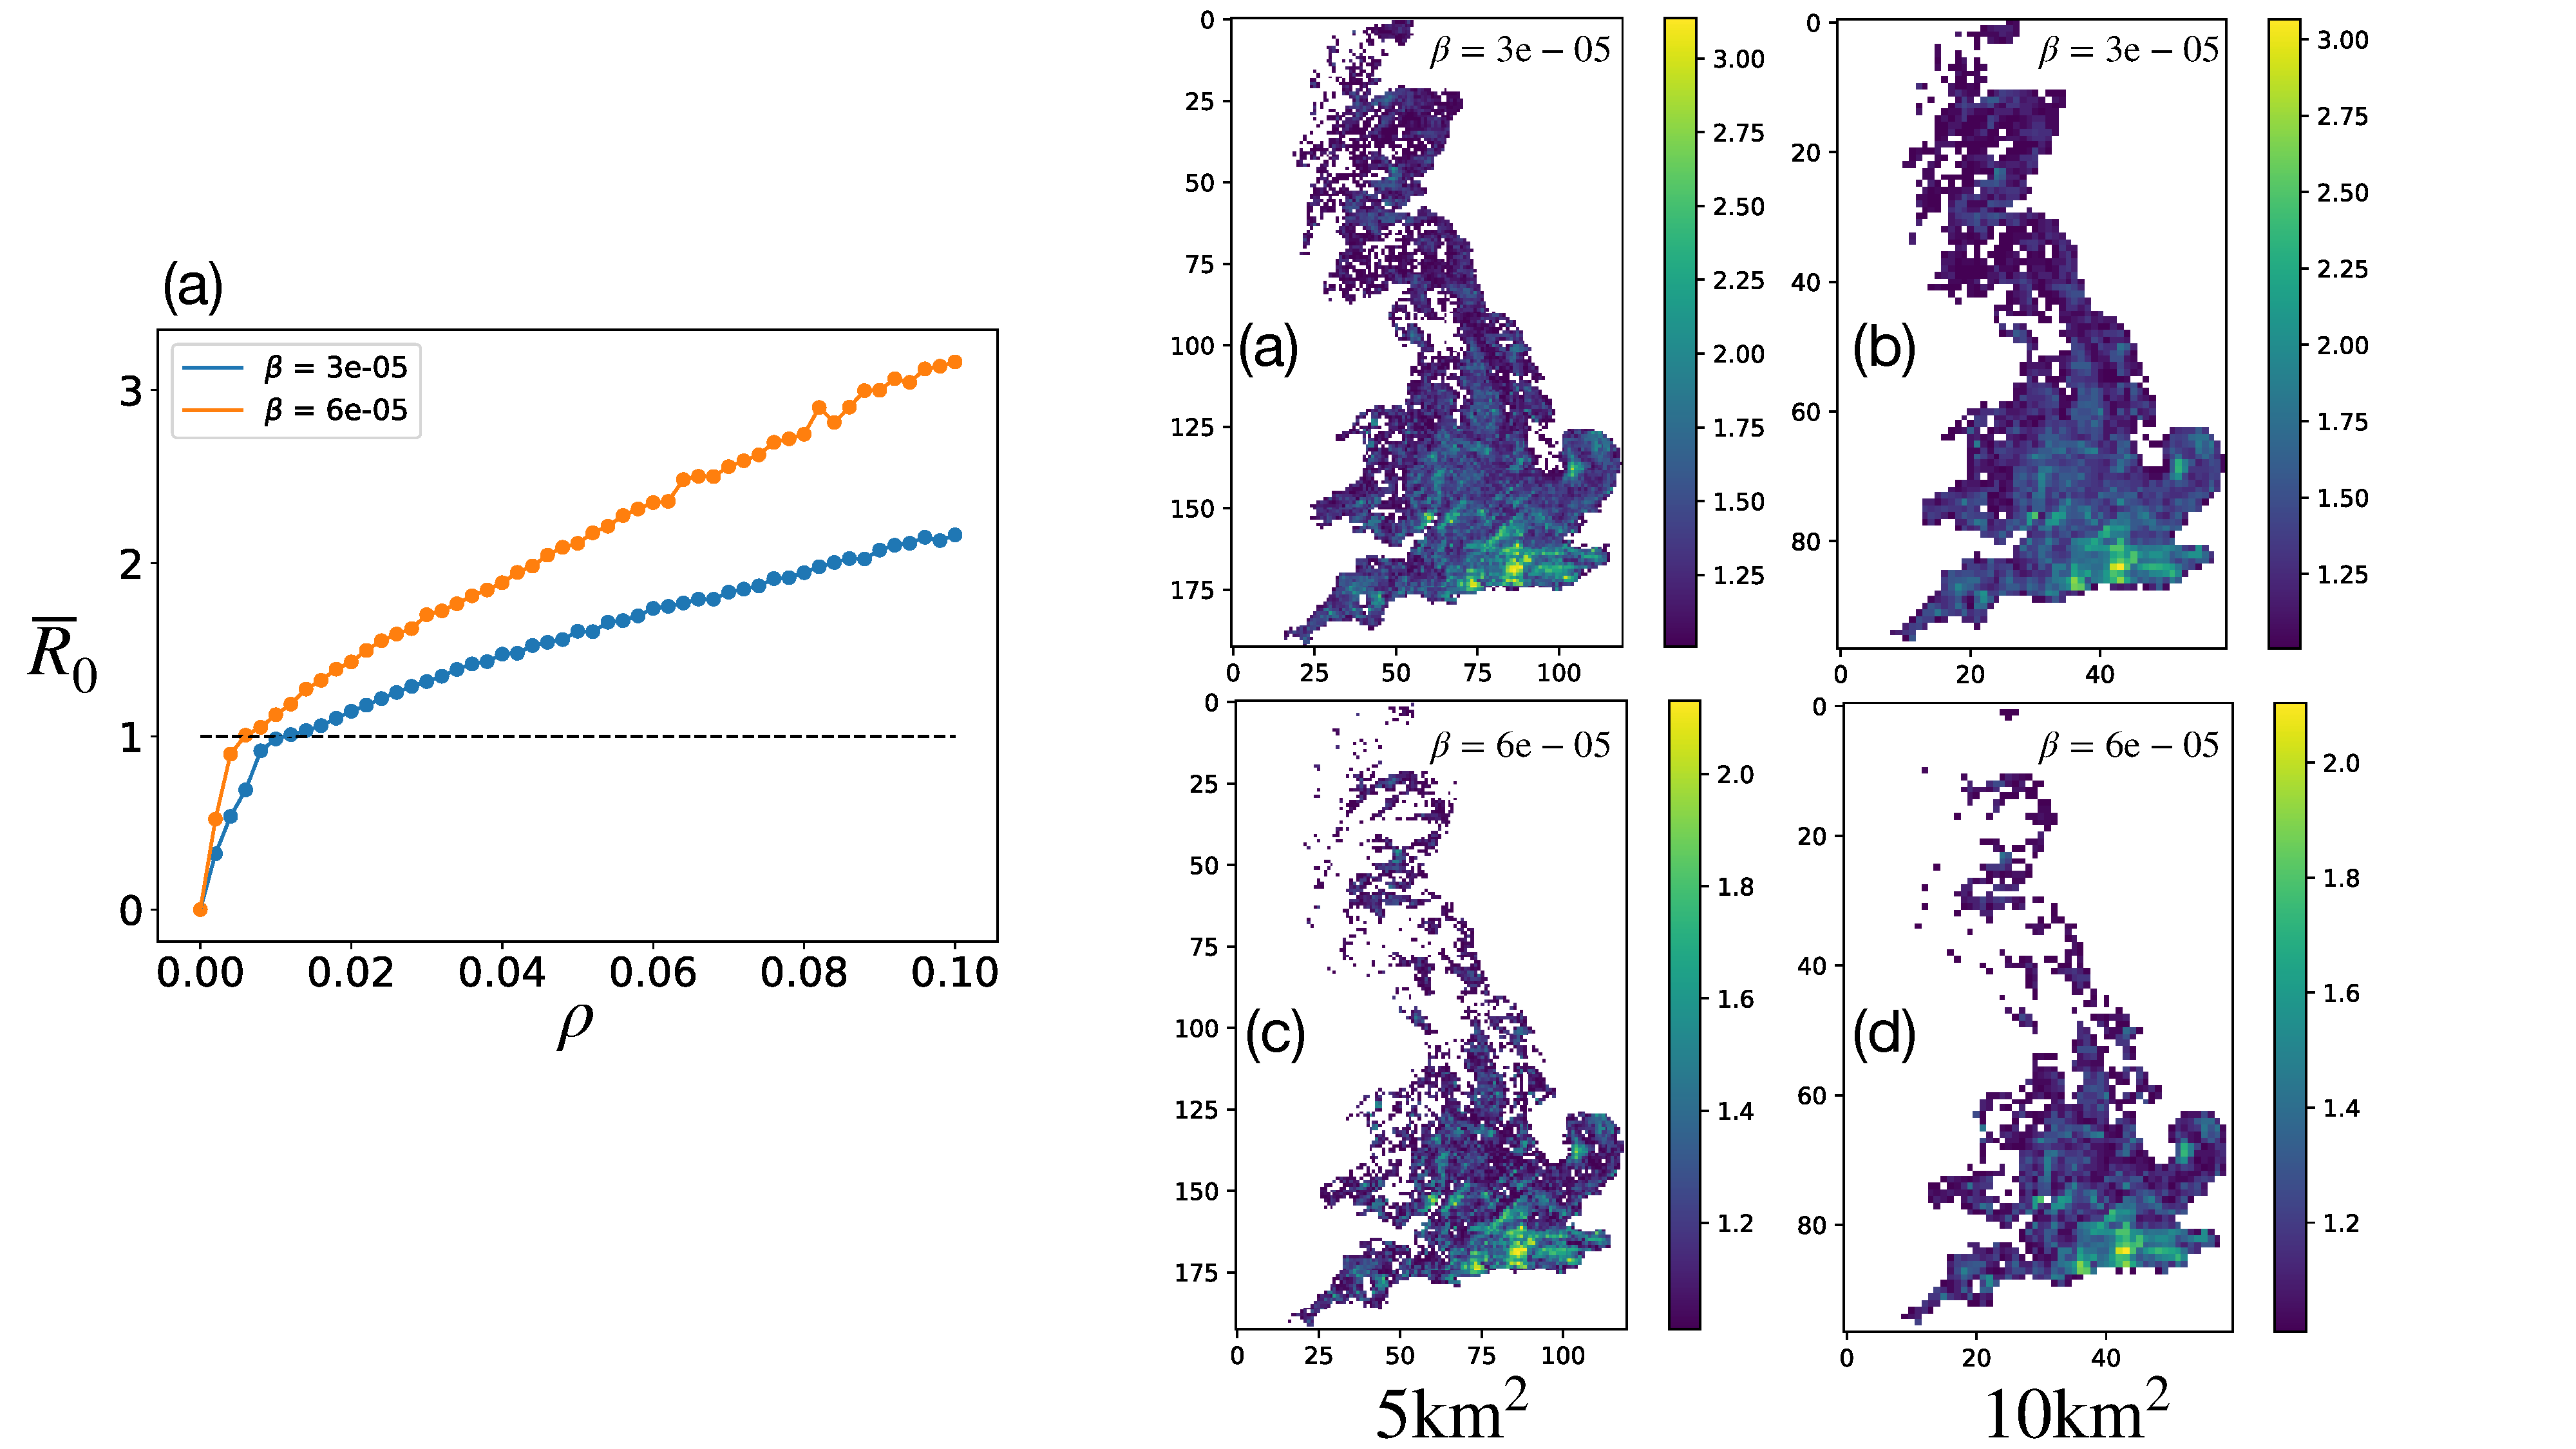
\includegraphics[scale=0.25]{chapter6/figures/fig2.pdf}
      \caption{(a) Ensemble-averaged $R_0$ between two values of $\beta$, for Gaussian dispersal of $\ell=1.6\mathrm{km}$. (a-b) $R_0$-map for $\beta=3\mathrm{e}-05$, coarse-grained at $5$, $ 10\mathrm{km^2}$. (c-d) $R_0$-map for $\beta=6\mathrm{e}-05$.}
    \label{fig:my_label}
\end{figure}
